\chapter{Denoising EDMR spectra}\label{ch:edmr}

\section{Introduction and project aim}
Electrically detected magnetic resonance (EDMR) measures changes in the current through a device when a magnetic resonance condition is reached. The resulting spectrum provides information about spin-dependent processes in the material. In practice, the measured response also depends on the sample and measurement circuit~\cite{leite2013}. The aim of this project is to investigate whether a neural network can recover an ideal spectrum from a noisy measurement without removing resonance features. The general idea is to create a synthetic dataset of clean spectra, add controlled noise and drift, train a model using this dataset, and compare its output with the known clean signal. The model is also compared with traditional denoising techniques. Synthetic data are useful at this stage because the correct answer is known for every spectrum, including spectra with overlapping peaks.

\section{Creating the synthetic dataset}\label{sec:data}
\subsection{Clean spectra}
First we start with an index grid $x=0,1,\ldots,1023$. An individual component has the shape
\begin{equation}
 f(x)=a(x-b)\exp\left[-c(x-b)^2\right],\qquad c>0.
 \label{eq:peak}
\end{equation}
This is proportional to the derivative of a Gaussian. It is a simple surrogate for an EDMR resonance feature. Each clean spectrum is the sum of $K$ resonance features,
\begin{equation}
 y(x)=\sum_{k=1}^{K} f_k(x),\qquad K\in\{1,2,3,4,5\}.
\end{equation}
The number of components is sampled uniformly. For each component, the width parameter $w$ is sampled uniformly between 0 and 40 sample intervals, and its individual lobe height $h$ is sampled uniformly between 0 and 1.5. For $w>0$, the parameters in Equation~\ref{eq:peak} are then set to
\begin{equation}
 a=\frac{h\exp(1/2)}{w},\qquad c=\frac{1}{2w^2}.
\end{equation}
An exactly zero-width component contributes zero on the sampled grid. The extrema occur at $x=b\pm w$, where the component has amplitudes $\pm h$. This makes the chosen width and height directly interpretable. The centre is drawn from $b\sim U(-40,1063)$, allowing peaks to extend beyond the scan boundaries. Overlap is allowed, so the extrema of the summed spectrum need not have the height of any individual component. Amplitudes are synthetic units, and $x$ has not been calibrated to magnetic field.

\subsection{Coloured-noise mixtures}
Each spectrum contains a random mixture of zero to five distinct noise colours. The colours and their power law exponents are shown in Table~\ref{tab:colours}. White noise is sampled from a Gaussian distribution. For the other colours, the real Fourier transform of a white-noise sequence is multiplied by a frequency-dependent amplitude weight,
\begin{equation}
 A(f)\propto f^{-\beta/2},\qquad P(f)\propto f^{-\beta},\qquad f>0.
\end{equation}
This Fourier-weighting approach is described in the coloured-noise implementation example linked in the notebook~\cite{bob2021noise}. The zero-frequency coefficient is set to zero. After the inverse transform, the coloured component has its mean subtracted and is multiplied by a factor that gives it the sampled standard deviation.

\begin{table}[htbp]
\centering
\begin{tabular}{lrl}
\toprule
Colour & $\beta$ & Relative emphasis\\
\midrule
Brown & 2 & Low frequencies\\
Pink & 1 & Low frequencies\\
White & 0 & Flat power spectrum\\
Blue & $-1$ & High frequencies\\
Violet & $-2$ & High frequencies\\
\bottomrule
\end{tabular}
\caption{Noise colours implemented in the notebook. The mixture need not follow one power law.}
\label{tab:colours}
\end{table}

The selected components receive independent strength settings from $U(0,1.0)$ and are summed. The resulting mixture is centred and rescaled to an overall standard deviation $\sigma\sim U(0,0.4)$. The relative mixture strengths and total noise level therefore vary separately. Zero selected components or zero total strength produce no random noise. Each sample has fixed noise once the dataset is created; the noise is not regenerated at every training epoch.

\subsection{Baseline drift}
A separate smooth baseline is added to 80\% of the spectra. The remaining 20\% have no added baseline drift. Let $u$ run uniformly from 0 to 1 across the scan, and let $t=2u-1$. The drift is
\begin{equation}
 d(x)=d_0+d_1t+d_2\left(t^2-\overline{t^2}\right)
       +A\sin(2\pi\nu u+\phi).
 \label{eq:drift}
\end{equation}
The offset and slope are each drawn uniformly between $-0.3$ and $0.3$. Curvature lies between $-0.2$ and $0.2$, the sinusoidal amplitude between 0 and 0.15, and the number of cycles between 0 and 1.5. Phase is uniform between 0 and $2\pi$. These are starting values for a controlled synthetic experiment. Their distributions have not been estimated from real measurements. The baseline is not centred after construction, because the offset is one of the unwanted contributions the model is intended to remove.

The corrupted input is
\begin{equation}
 z(x)=y(x)+n(x)+d(x),
\end{equation}
where $n$ is the coloured-noise mixture. The target remains $y(x)$, so both noise and baseline drift must be removed. Figure~\ref{fig:dataset} illustrates the generated contributions.

\begin{figure}[htbp]
\centering
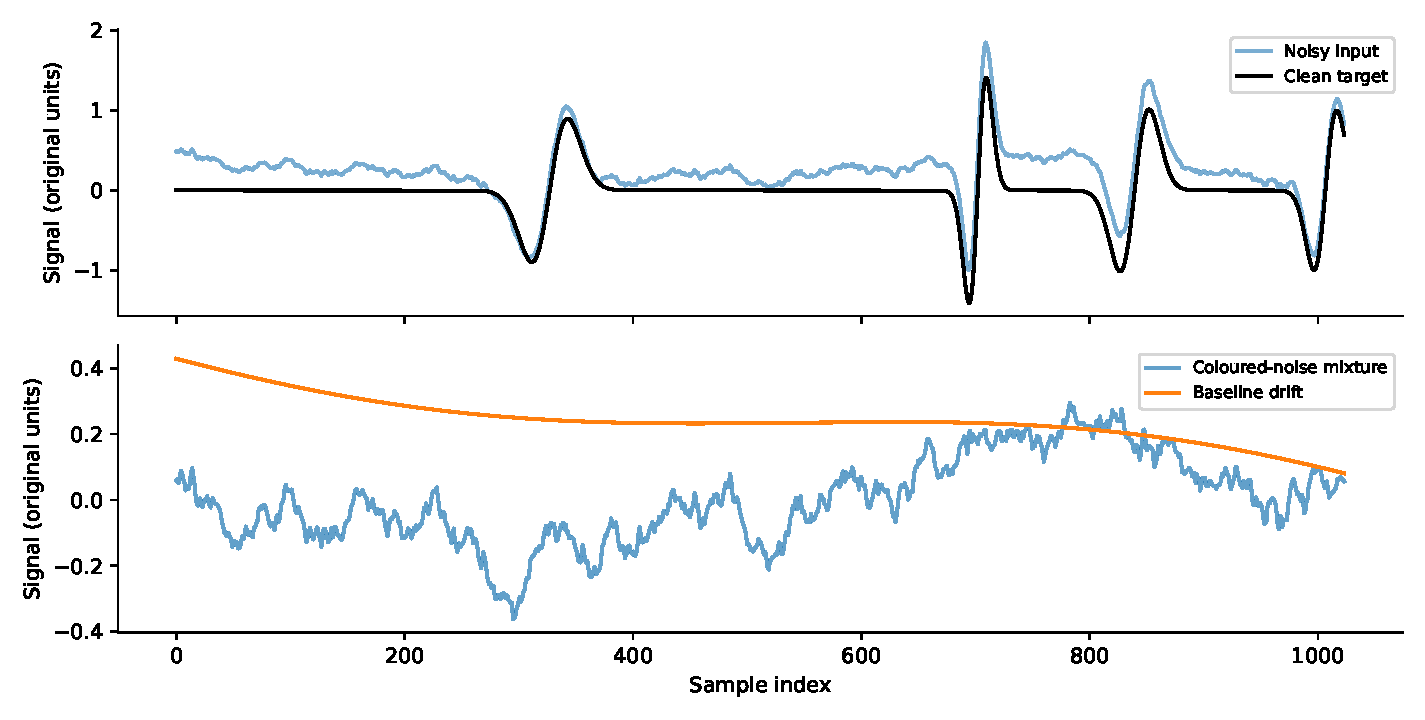
\includegraphics[width=0.94\textwidth]{figures/dataset_example.pdf}
\caption{A synthetic example generated from the current data functions with illustration seed 12345. The upper panel shows the clean target and corrupted input; the lower panel separates the coloured-noise mixture and baseline drift. This is a data-generation illustration, not a network reconstruction.}
\label{fig:dataset}
\end{figure}

\subsection{Normalisation and data splits}
The input amplitude is normalised separately for each spectrum. The scale is the larger of the 95th percentile of the absolute corrupted input and one-tenth of its maximum absolute amplitude,
\begin{equation}
 s_i=\max\left[Q_{0.95}\!\left(|z_i|\right),\frac{\max_j|z_{ij}|}{10}\right],\qquad
 \widetilde z_i=\frac{z_i}{s_i},\qquad \widetilde y_i=\frac{y_i}{s_i}.
 \label{eq:normalisation}
\end{equation}
If the scale is zero, it is set to 1. A very narrow, noise-free peak can have a nearly zero 95th percentile even when its amplitude is large. The maximum-amplitude term prevents the normalised input from becoming extremely large and overflowing the training loss. The target uses the same input-derived scale; it is not independently normalised. This avoids requiring the unknown clean amplitude when processing a real measurement. No mean subtraction or clipping is applied to the spectrum. The scale is retained so that the predicted clean spectrum can be returned to the original amplitude units.

The code generates 50,000 training spectra with seed 10, 2,000 validation spectra with seed 20, and 2,000 test spectra with seed 30. Training batches are shuffled with a PyTorch generator seeded at 42. Validation and test batches are not shuffled. Validation data select the checkpoint and traditional-filter settings. The test set is used for the final evaluation and reconstruction plots.

\section{The neural network}
\subsection{Residual one-dimensional U-Net}
The model is a one-dimensional adaptation of the encoder-decoder design introduced in U-Net~\cite{ronneberger2015}. The encoder reduces the spatial resolution to learn broader patterns, and the decoder restores the original resolution. At each decoder level, features from the matching encoder level are concatenated with the upsampled features. These skip connections provide a route for fine spectral information around the compressed representation.

The network predicts an additive unwanted contribution $r_\theta$, and returns
\begin{equation}
 \widehat{\widetilde y}=\widetilde z-r_\theta(\widetilde z).
 \label{eq:residual}
\end{equation}
Predicting the unwanted contribution follows the residual-denoising idea used in DnCNN~\cite{zhang2017}. Here the residual includes both the random noise and the added drift. The model is supervised through the clean output in Equation~\ref{eq:residual}; the residual is not given a separate training loss. The final output layer has no activation, allowing the residual to have either sign. Its weights and bias are initially zero, so the untrained model starts as an identity mapping.

Each convolution block contains two one-dimensional convolutions with kernel size 7 and padding 3. A ReLU follows each convolution. Average pooling halves the length between encoder levels. The decoder uses linear interpolation to the matching encoder length, a kernel-size-1 projection, concatenation with the skip features, and another convolution block. The channel counts are 16, 32, 64 and 128. The model has 352,177 trainable parameters. Figure~\ref{fig:architecture} shows the implemented structure for a 1,024-point input.

\begin{figure}[htbp]
\centering
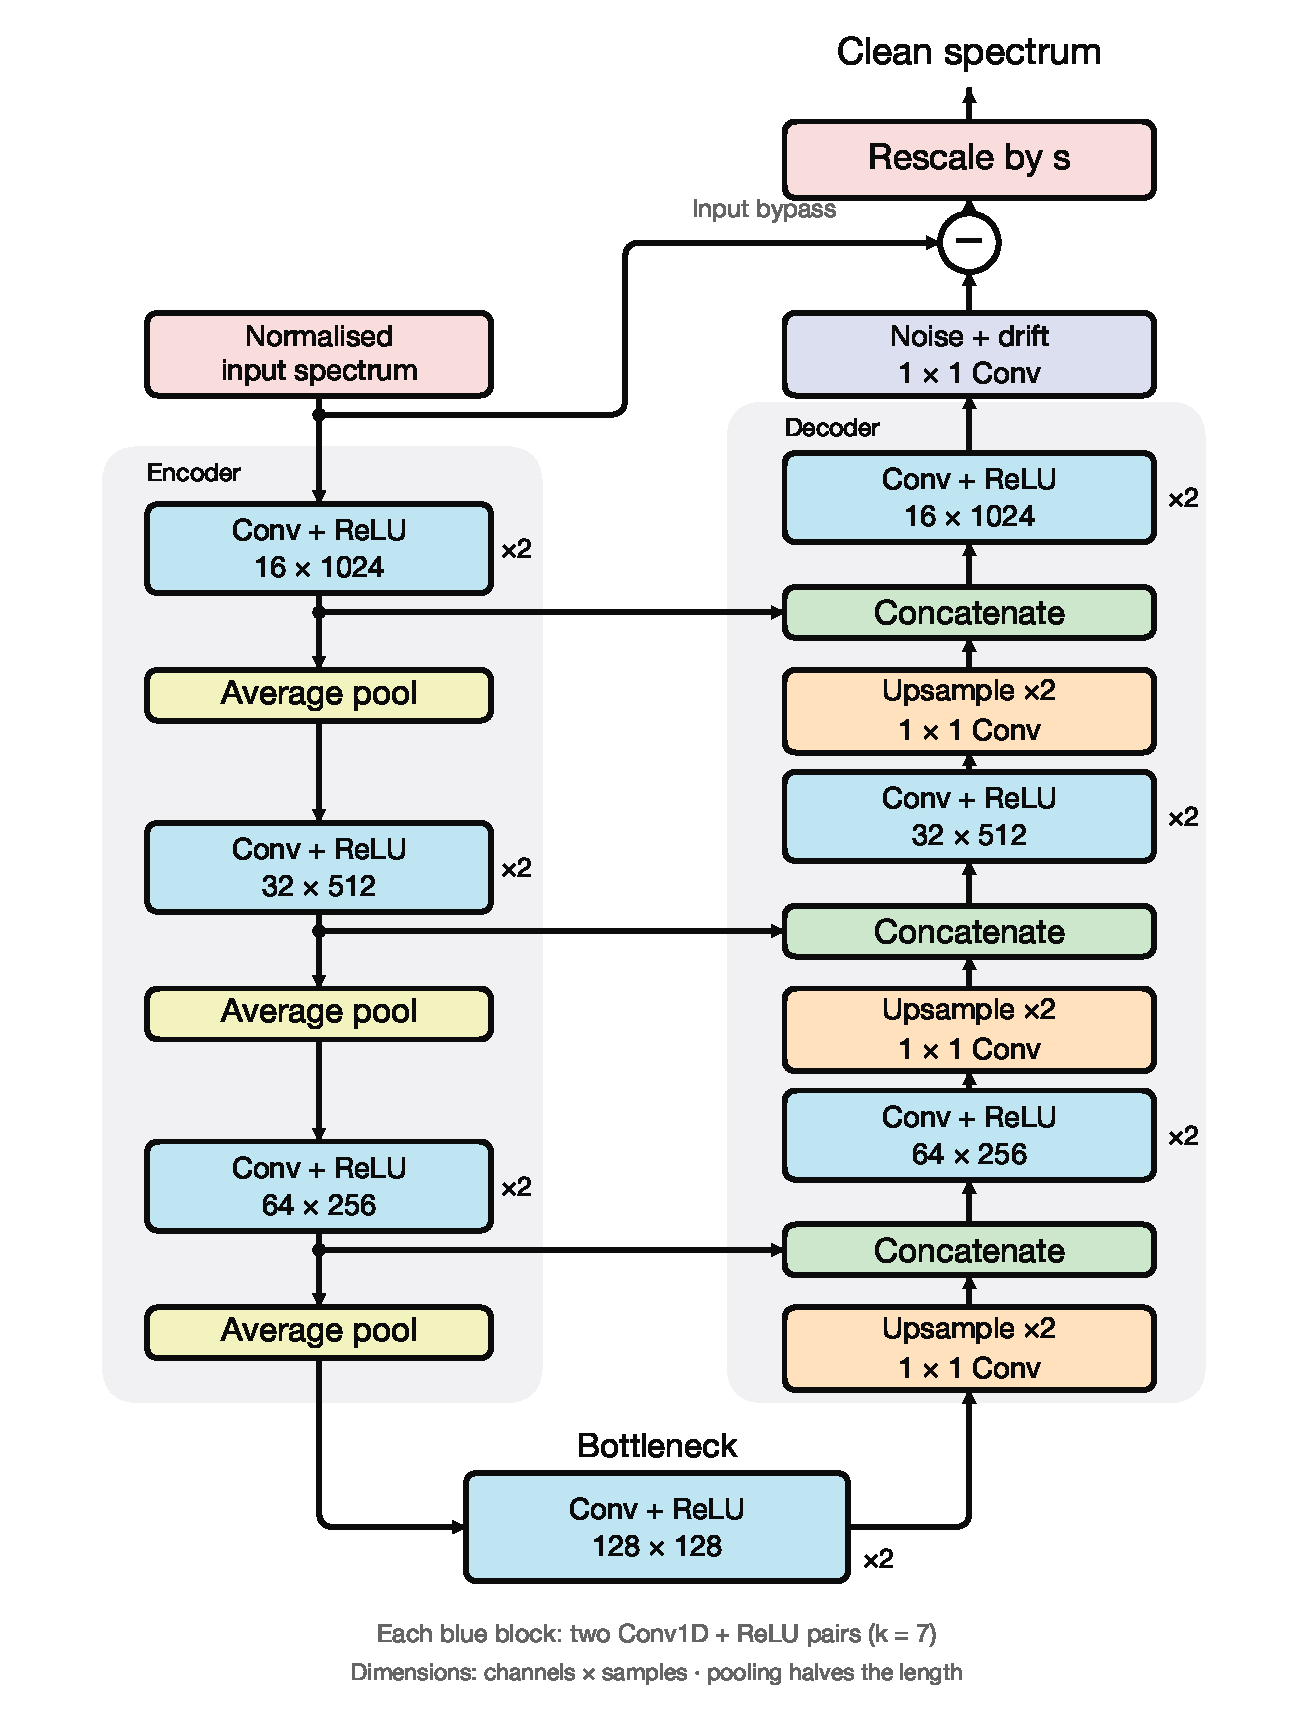
\includegraphics[width=0.86\textwidth,height=0.76\textheight,keepaspectratio]{figures/unet_architecture.pdf}
\caption{The implemented residual 1D U-Net. Dimensions are output channels $\times$ sequence length. Each blue block contains two Conv1D--ReLU pairs in series, with separate learned weights. Horizontal skip connections concatenate matching encoder features. The final kernel-size-1 convolution predicts noise and drift; subtraction and inverse scaling give the clean prediction in original amplitude units. AI assistance was used to construct this diagram.}
\label{fig:architecture}
\end{figure}

The final output in original units is obtained by multiplying by the saved input scale,
\begin{equation}
 \widehat y_i=s_i\widehat{\widetilde y}_i.
\end{equation}
The removed baseline is not added back. The inference helper accepts one raw spectrum or a batch and applies this same preprocessing and inverse scaling.

\subsection{Loss, optimiser and early stopping}
The training loss is the mean squared error (MSE) between the normalised prediction and target. For $M$ spectra with $N=1024$ points,
\begin{equation}
 \mathcal L=\frac{1}{MN}\sum_{i=1}^{M}\sum_{j=1}^{N}
 \left(\widehat{\widetilde y}_{ij}-\widetilde y_{ij}\right)^2.
 \label{eq:mse}
\end{equation}
A smaller value indicates a closer match to the known target, and zero would indicate a perfect pointwise reconstruction. Normalised MSE weights the original squared errors by $1/s_i^2$, so it is not the same quantity as original-unit MSE. The model is trained in PyTorch with Adam~\cite{kingma2015} at a learning rate of $10^{-3}$ and a batch size of 128. The maximum is 40 epochs. Early stopping is applied when validation MSE has not improved by more than $10^{-5}$ relative to the patience reference for six epochs. The best validation weights are saved independently of this threshold and restored at the end. Training uses gradient updates; validation uses evaluation mode without gradient tracking. The model was trained on Apple's MPS.

\subsection{Traditional methods}
The model is compared with a moving average~\cite{scipyuniform}, Gaussian smoothing~\cite{scipygaussian}, Savitzky-Golay smoothing~\cite{scipysavgol}, polynomial baseline correction, and polynomial baseline correction followed by Savitzky-Golay smoothing. The smoothing methods average nearby samples or fit a local polynomial. Baseline correction fits a polynomial across the noisy scan and subtracts it before any smoothing. It uses only the noisy input, not the clean target.

Each method is tuned using normalised validation MSE. Moving-average and Savitzky-Golay windows are chosen from 5, 11, 21, 41, 81 and 121 samples. Gaussian widths are chosen from 1, 2, 4, 8, 16 and 24 samples. Savitzky-Golay polynomial orders are 2 or 3, and baseline degrees are 0, 1, 2 or 3. The settings in Table~\ref{tab:settings} are then fixed for test evaluation.

\begin{table}[htbp]
\centering
\begin{tabularx}{\textwidth}{@{}lX@{}}
\toprule
Method & Selected settings\\
\midrule
Moving average & Window 11 samples\\
Gaussian smoothing & Standard deviation 4 samples\\
Savitzky-Golay & Window 21 samples; polynomial order 2\\
Polynomial baseline & Degree 3\\
Baseline + Savitzky-Golay & Baseline degree 3; window 21 samples; order 2\\
\bottomrule
\end{tabularx}
\caption{Traditional-method settings selected using validation data.}
\label{tab:settings}
\end{table}

\section{Current results}\label{sec:results}
\subsection{Training history}
The training run completed in 26 epochs and restored the epoch-23 checkpoint selected using the internal normalised validation loss. Its validation MSE in original amplitude units is 0.002015. The saved training history is shown in Figure~\ref{fig:loss}. Reported MSE values are in original amplitude units squared and are rounded to six decimal places.

\begin{table}[htbp]
\centering
\begin{tabular}{lrr}
\toprule
Quantity & Training MSE & Validation MSE\\
\midrule
Epoch 1 & 0.018661 & 0.003940\\
Restored epoch 23 & 0.001841 & 0.002015\\
Final epoch 26 & 0.001769 & 0.002171\\
\bottomrule
\end{tabular}
\caption{MSE in original amplitude units squared from the training run. Training error is accumulated during parameter updates; validation error is measured after each epoch.}
\label{tab:training}
\end{table}

The error falls rapidly at the start of training and then improves more slowly. Between epochs 23 and 26, training loss decreases while validation loss fluctuates above its minimum. This is consistent with diminishing generalisation benefit and late overfitting. Early stopping limits further training when validation performance stops improving.

\begin{figure}[htbp]
\centering
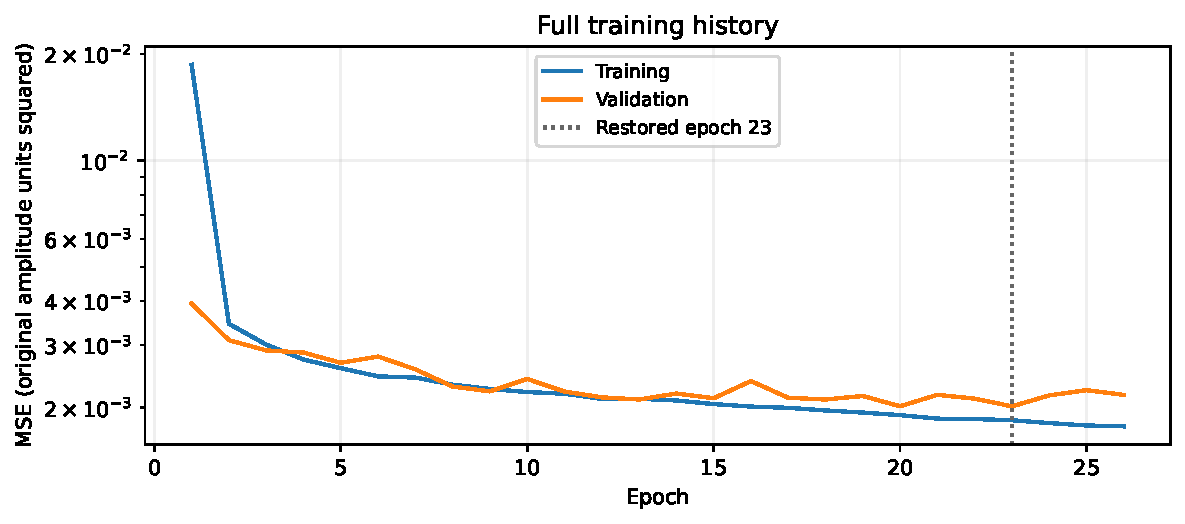
\includegraphics[width=\textwidth]{figures/training_history.pdf}
\caption{Training and validation MSE in original amplitude units squared versus epoch. The full training history is shown on a logarithmic axis. The dotted line marks the restored epoch-23 checkpoint.}
\label{fig:loss}
\end{figure}

\subsection{Test evaluation and comparison with the corrupted input}
The restored model is evaluated on the 2,000 unseen test spectra. Its test MSE is 0.002039 in original amplitude units squared, compared with 0.081426 for the unprocessed input. The input and prediction are compared with the same clean target after reversing the input normalisation. The test set does not select the checkpoint or filter settings, so this is an unseen test set evaluation.

\subsection{Example reconstructions}
Figure~\ref{fig:reconstruction} compares the network with polynomial baseline correction followed by Savitzky-Golay smoothing on the first three test spectra (indices 0, 1 and 2). These fixed examples were not selected for good results. Predictions have been de-normalised, so the curves can be compared in the original synthetic amplitude units. The predictions suppress substantial noise and drift. In the second and third examples, the predicted and clean curves are close over much of the resonance feature. The first example still shows amplitude differences, baseline wiggles and a false peak where the clean target is flat. These examples support qualitative reconstruction of the generated features, but also show why a low average MSE does not guarantee that every reconstructed peak is correct.

\begin{figure}[H]
\centering
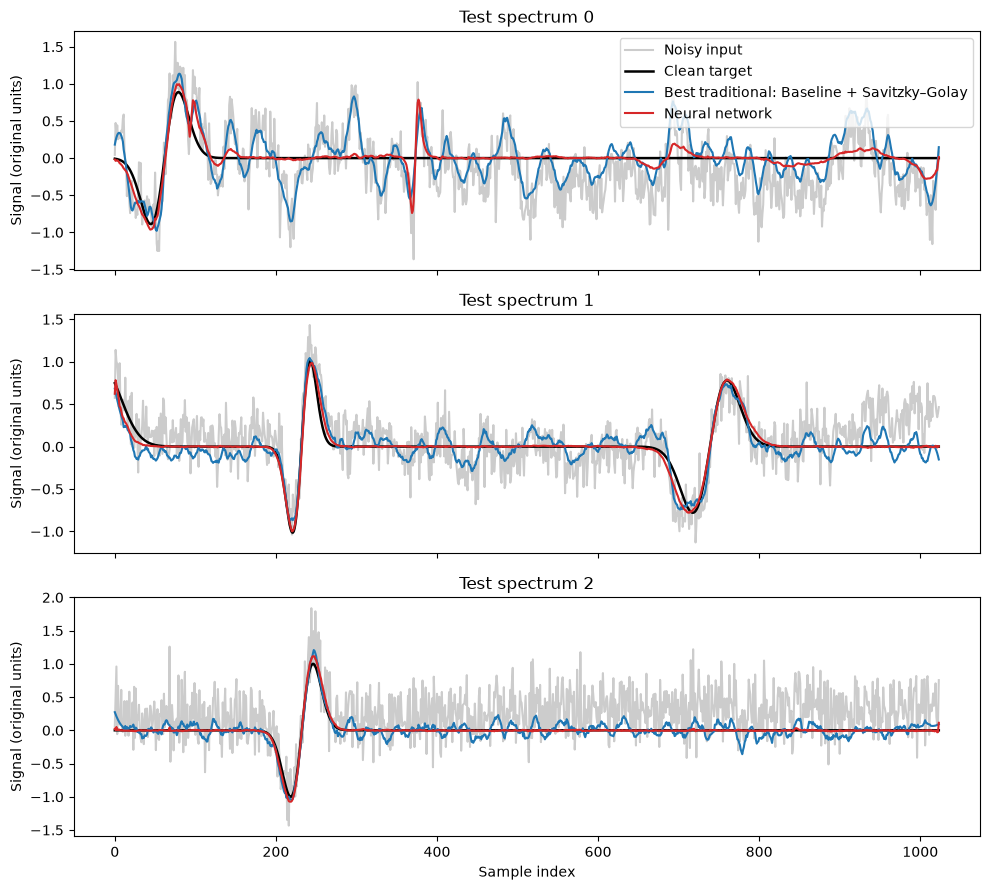
\includegraphics[width=0.94\textwidth,height=0.63\textheight,keepaspectratio]{figures/test_method_comparison.png}
\caption{Comparison on test spectra 0, 1 and 2 from the notebook. Grey is the corrupted input, black is the clean target, blue is polynomial baseline correction followed by Savitzky-Golay smoothing, and red is the restored epoch-23 network output. All curves are in original synthetic amplitude units; traditional-filter settings were selected using validation data.}
\label{fig:reconstruction}
\end{figure}

\subsection{Comparison with traditional techniques}
Table~\ref{tab:comparison} compares every method on the same test spectra. Polynomial baseline correction followed by Savitzky-Golay smoothing is the strongest traditional method by MSE. Its original-unit MSE is 0.015177, compared with 0.002039 for the neural network. Figure~\ref{fig:comparison} shows the original-unit errors.

\begin{table}[H]
\centering
\begin{tabularx}{\textwidth}{@{}Xr@{}}
\toprule
Method & MSE\\
\midrule
Noisy input & 0.081426\\
Moving average & 0.052340\\
Gaussian smoothing & 0.051858\\
Savitzky-Golay & 0.052813\\
Polynomial baseline & 0.043791\\
Baseline + Savitzky-Golay & 0.015177\\
Neural network & 0.002039\\
\bottomrule
\end{tabularx}
\caption{MSE in original amplitude units squared on the same 2,000 held-out test spectra. Values are rounded from the current notebook's saved comparison table.}
\label{tab:comparison}
\end{table}

\begin{figure}[htbp]
\centering
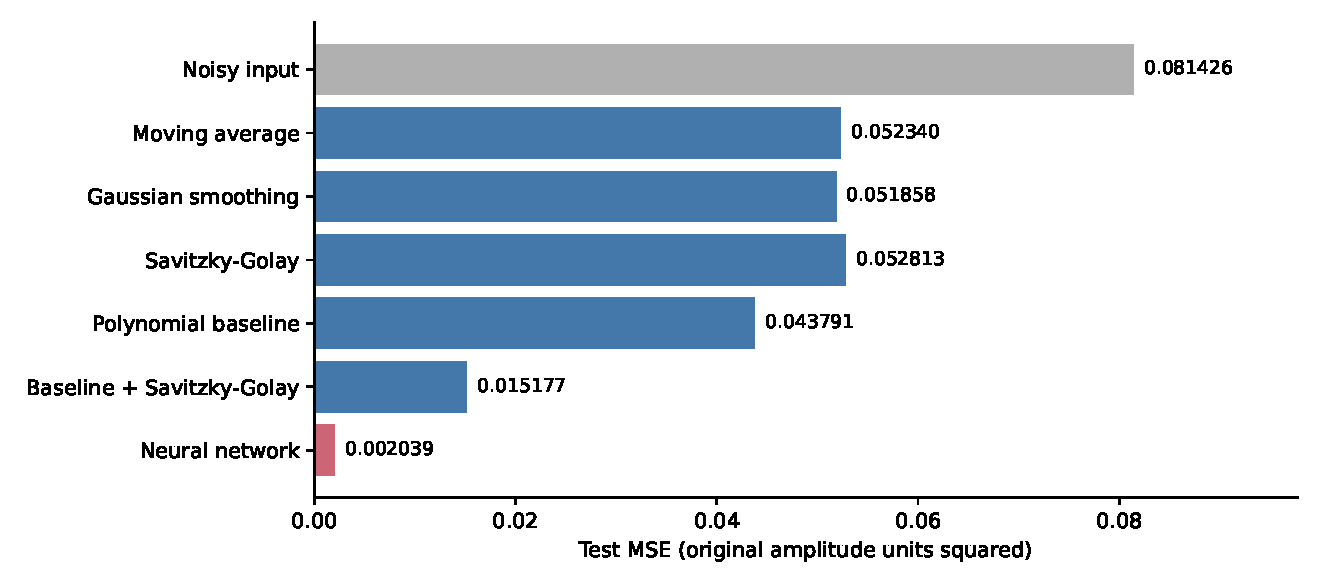
\includegraphics[width=0.95\textwidth]{figures/traditional_comparison.pdf}
\caption{Original-unit MSE on the same held-out test set. Lower values mean closer agreement with the clean target.}
\label{fig:comparison}
\end{figure}

\section{Discussion and remaining validation}\label{sec:discussion}
\subsection{Peak preservation and limitations of MSE}
Pointwise MSE is a useful overall measure, but it does not directly report errors in peak position, lobe height or linewidth. Error over many near-baseline samples can dominate the average metric, while an isolated false peak can still be important. The next evaluation should quantify these feature errors. A peak-preserving loss or explicit line fitting may be worth investigating. An alternative model trained to predict the input feature parameters, such as feature position, lobe height and linewidth, is also worth investigating. These are continuous parameters, so this would be a regression task; discrete properties such as peak count could be treated as classification.

\subsection{Comparison with traditional methods}
The test comparison shows lower aggregate errors for the network than for the five traditional methods tested here. Baseline correction improves the traditional smoothing result substantially, because smoothing alone leaves slow drift. A baseline polynomial can also remove part of a broad or edge-truncated resonance. The comparison covers a finite search of filter settings on one synthetic distribution. It does not show that the network is better than every traditional method or that the same advantage will hold for measured spectra.

The results are from one training run. Repeated training seeds would help assess their variability.

\subsection{Application to measured EDMR spectra}
For measured spectra, the input should be represented on a known, consistently ordered magnetic-field grid. The network currently operates on sample indices, so its notion of width is in points. A physical width $w_B$ corresponds to approximately $w_B/\Delta B$ sample intervals when the field spacing is $\Delta B$. Changing the number of points without accounting for the field spacing can therefore change the features seen by the model. A practical application should use compatible sampling or retrain the generator using representative physical widths. Merely resampling every scan to 1,024 points does not establish that the inputs match the training distribution.

Amplitude normalisation is already included, but it does not correct all differences between synthetic and measured data. Real line shapes, measurement phase, resonances near scan boundaries, and the noise and drift distributions need to be represented. The generator now allows edge-truncated components, but uses only one derivative-Gaussian family with positive component coefficients, and does not simulate quadrature channels or signal-dependent shot noise. These assumptions limit the present scope. A useful real-data validation would compare individual noisy scans with an independently acquired higher-SNR reference, while checking that denoising does not alter fitted feature parameters. Reference acquisition and scan alignment also need to be considered. No measured EDMR spectrum has been processed or validated in the current notebook.

\section{Conclusion}
The current project implements an end-to-end synthetic denoising pipeline with variable peak counts and strengths, mixed coloured noise, smooth baseline drift, shared input-derived normalisation, and a residual 1D U-Net. The trained model restored an epoch-23 checkpoint after stopping at epoch 26. Its validation MSE is 0.002015 and its test MSE is 0.002039, both in original amplitude units squared. The example predictions show substantial removal of the generated corruption, with local reconstruction errors still visible in the first test spectrum.

The experiment is a working synthetic proof of concept. On the held-out test set, the network has an MSE of 0.002039, compared with 0.015177 for polynomial baseline correction followed by Savitzky-Golay smoothing, the strongest traditional method tested. Future experiments are quantitative measures of peak preservation, a model that predicts peak parameters, repeated training seeds, and validation on real EDMR scans.
